\documentclass[draft=false]{oblivoir}
\author{Moon Il-chul \\ \href{mailto:icmoon@kaist.ac.kr}{icmoon@kaist.ac.kr} 
   \and Shin Seung-jae \\ \href{mailto:tmdwo0910@kaist.ac.kr}{tmdwo0910@kaist.ac.kr} }
\setcounter{chapter}{14}
\title{Chapter 14. Artificial Neural Network}
\usepackage{indentfirst}
\usepackage{graphicx}
\graphicspath{ {Figure/} }
\usepackage{hyperref}
\usepackage{amsmath}
\usepackage{amssymb}
\usepackage{amsfonts}
\usepackage{dsfont}
\usepackage[]{algorithm2e}
\usepackage{chngcntr}
\counterwithin{figure}{chapter}
\setcounter{tocdepth}{2}
\setcounter{secnumdepth}{3}
\hypersetup{pdfborder={0 0 0}}
\renewcommand{\thefigure}{\thechapter-\arabic{figure}}
\renewcommand{\theequation}{\thechapter.\arabic{equation}}
\newlength\myindent
\setlength\myindent{5em}

\begin{document}
\maketitle
\tableofcontents
\section{Perceptron and Neural network}
%-----------------------------------------------------------------
딥러닝은 머신러닝의 한 분야로서  인공신경망 (Artificial Neural Network)에 기반한 기계학습 기법이라고 할 수 있다. 바야흐로 딥러닝의 시대라 부를만큼 최근 딥러닝에 대한 관심이 높아짐에 따라 자연스럽게 인공 신경망에 대한 관심도 높아지고 있는데, 이번 장에서는 인공신경망의 초기 형태인 Feed-forward Neural Network에서부터 최근 다양한 형태로 변화된 인공신경망까지 함께 알아보고자 한다. 
\subsection{Artificial Neuron}
%-----------------------------------------------------------------
뉴런은 신경계와 신경조직을 이루는 기본 단위세포로서, 전기적, 화학적 신호를 통해 신체 내 다양한 자극 정보들을 전달하는 역할을 한다. 
\begin{figure}[ht] \centering 
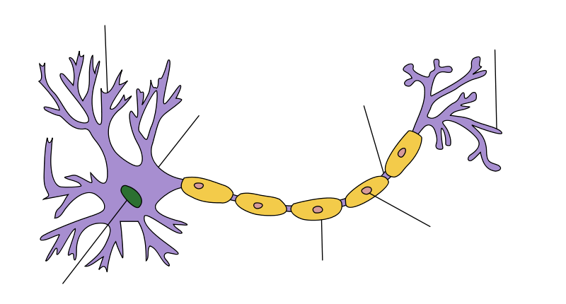
\includegraphics[scale=0.5]{fig14_1.png} 
\caption{뉴런의 구조}
\label{fig:14-1}
\end{figure}
이러한 뉴런의 역할 및 구조를 흉내내어, 인공적으로 만들어낸 것이 바로 인공 뉴런 (Artificial Neuron)이다. 결국 각각의 인공 뉴런은 정보를 전달 (Processing)하는 하나의 Unit이 되는데, 각각의 뉴런에 대한 정보의 입출력을 관할하는 activation 관계는 다음과 같이 나타낼 수 있다. 
\begin{equation}
a_{k}(X) = \sum_{0 \leq i \leq n}w_{ki}x_{i}, y_{k} = g(a_{k})
\label{eq:14-2-1}
\end{equation}
해당 뉴런으로 모이는 각각의 input $x_{i}$를 processing하기 위해 각각의 input에 해당하는 weight $w_{ki}$를 설정해주었고 이를 Linear Sum 형태로 표현해주었다. 

\begin{figure}[ht] \centering 
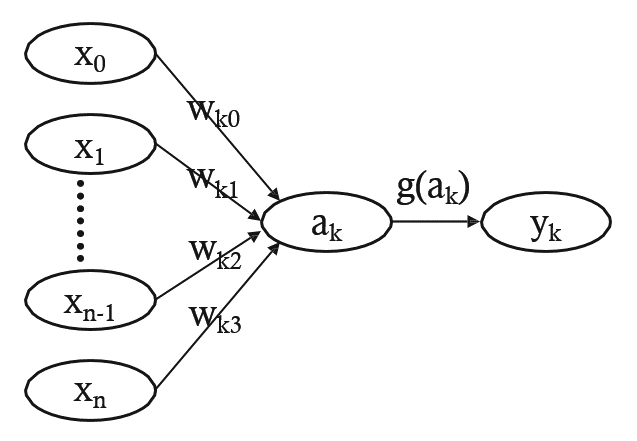
\includegraphics[scale=0.5]{fig14_2.png} 
\caption{인공 뉴런 (artificial neuron)의 구조}
\label{fig:14-2}
\end{figure}

또한 Linear sum 결과인 $a_{k}$에 대하여 임의의 activation function g를 통해 변환시킨 $g(a_{k})$, 즉 $y_{k}$가 output으로 나오게 된다. output activation function g로는 다양한 function을 활용할 수 있는데 대표적으로 Sigmoid function과 Rectified linear function 등이 있다.

간단히 말해, 인공 뉴런 (Artificial neuron)은 각기 다른 input 정보를 각각의 weight에 대한 linear sum으로 합쳐주는 input activation과 그 결과값을 한번 더 변환시켜주는 Output activation의 과정을 수행하는 구조라 할 수 있다. 

\subsection{Neuron Input Activation}
%-----------------------------------------------------------------
인공 뉴런 (artificial neuron)에서 각기 다른 input 정보를 linear sum 형태로 합쳐주는 input activation 과정에 대해 더 자세히 알아보자. 
\begin{equation}
a_{k}(X) = \sum_{0 \leq i \leq n}w_{ki}x_{i}
\label{eq:14-2-2}
\end{equation}
결국 i는 input feature의 dimension을 나타내며 k는 해당 뉴런, 즉 k번째 뉴런을 나타내는 index일 것이다. 또한 위의 선형식에 constant term 혹은 bias term을 넣어주기 위해 1의 값을 가지는 $x_{0}$와 $b_{k}$의 값을 가지는 $W_{ki}$ 를 추가로 introduce해주면 input activation 식을 아래와 같이 쓸 수 있다.  
\begin{equation}
a_{k}(X) = W^{T}_{k}X + b_{k}
\label{eq:14-2-3}
\end{equation}
마찬가지로 이를 k개의 neuron이 있는 Layer에 대한 식으로 일반화하면 아래와 같이 쓸 수 있다. 
\begin{equation}
A(X) = WX + B
\label{eq:14-2-4}
\end{equation}
이제 input activation function의 수식이 기하학적으로 어떤 의미를 갖는 지 아래의 그림을 통해 알아보도록 하자. input feature의 dimension이 3인 경우 식을 다음과 같이 쓸 수 있다. 
\begin{equation}
w_{1}x_{1} + w_{2}x_{2} + w_{3}x_{3} + b = 0 
\label{eq:14-2-5}
\end{equation}
아래의 그림과 같이 $\vec{w}$ $(w_{1},w_{2},w_{3})$은 dimension space 상에서  hyperplane의 orientation 방향을 결정짓는 변수이며 $b_{k}$의 경우 hyperplane의 위치를 조정하며 결정짓는 변수라 할 수 있는 것이다.
\begin{figure}[ht] \centering 
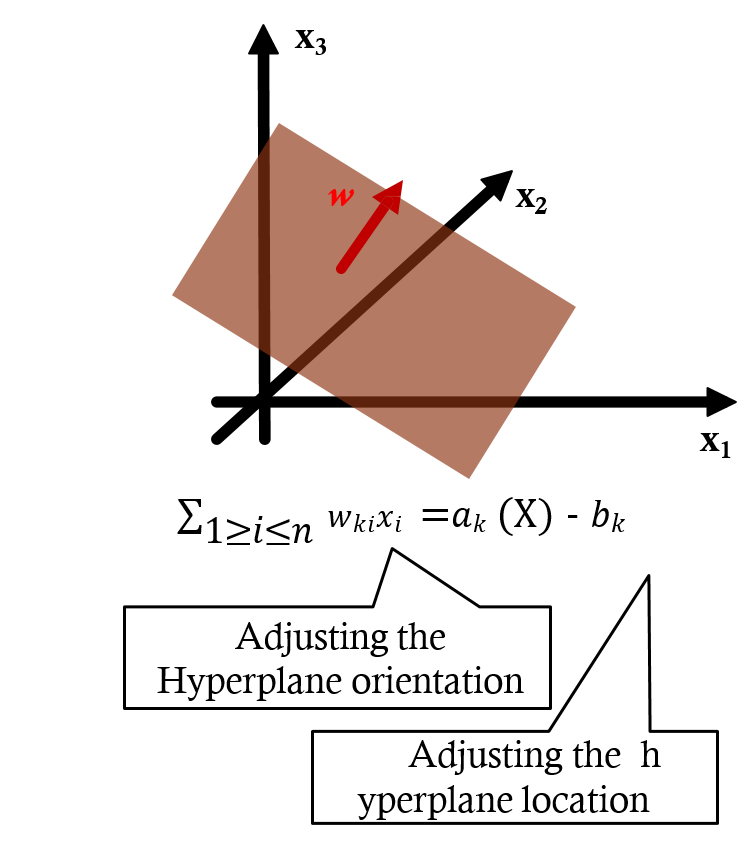
\includegraphics[scale=0.5]{fig14_3.png} 
\caption{input activation의 기하학적 의미}
\label{fig:14-3}
\end{figure}
\subsection{Neuron Output Activation Function}
%-----------------------------------------------------------------
이번에는 input activation이 완료된 input feature의 linear sum을 Output으로 변환하는 Output activation에 대해 더 자세히 알아보자.
\begin{equation}
g(a_{k}(X)) = y_{k}
\label{eq:14-2-6}
\end{equation}
위의 식에서 $a_{k}(X)$은 linear sum 결과값이며 이를 변환시켜주는 function g가 결국 output activation function이라 할 수 있다. 그 결과로 나오는 $y_{k}$가 바로 최종 Output이 될 것이다. Output Activation function은 뉴런들의 집합인 layer마다 각기 다른 종류의 function을 쓰기도 하는 등 그 종류와 목적이 매우 다양하다. 이러한 후보 function들 중 대표적으로 사용되는 sigmoid function을 예로 들어 설명해보도록 하겠다.
\begin{figure}[ht] \centering 
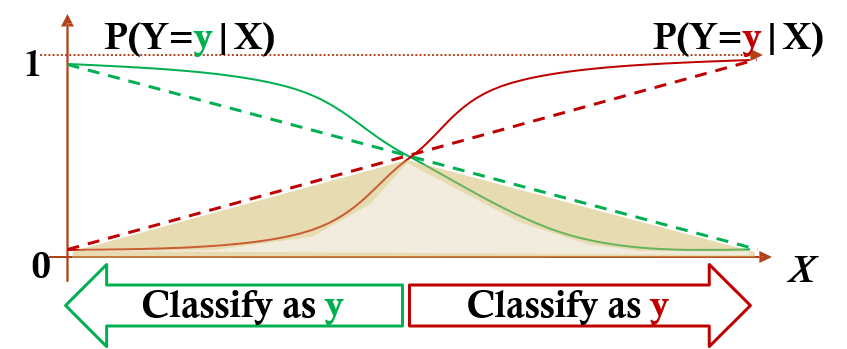
\includegraphics[scale=0.5]{fig14_4.png} 
\caption{Logistic regression과 linear regression간의 Bayes risk 차이}
\label{fig:14-4}
\end{figure}

Sigmoid function은 전 구간이 differential하면서 monotonically increasing하는 특징을 가지고 있는데, 대표적인 sigmoid function으로 logistic function을 꼽을 수 있다. 아래의 그림에서 볼 수 있듯이 logistic regression은 S-Curve의 모양을 띄고 있으며 이에 따라 분류 기준값에 대하여 sharply adapt하는 성질을 가지고 있다. 이를 통해 기존의 linear classifier (점선) 대비 bayes risk를 크게 감소시키는 방식의 classifier가 된 것이다. 이는 activation function의 조건에 잘 부합한다고 볼 수 있다. 
\begin{figure}[ht] \centering 
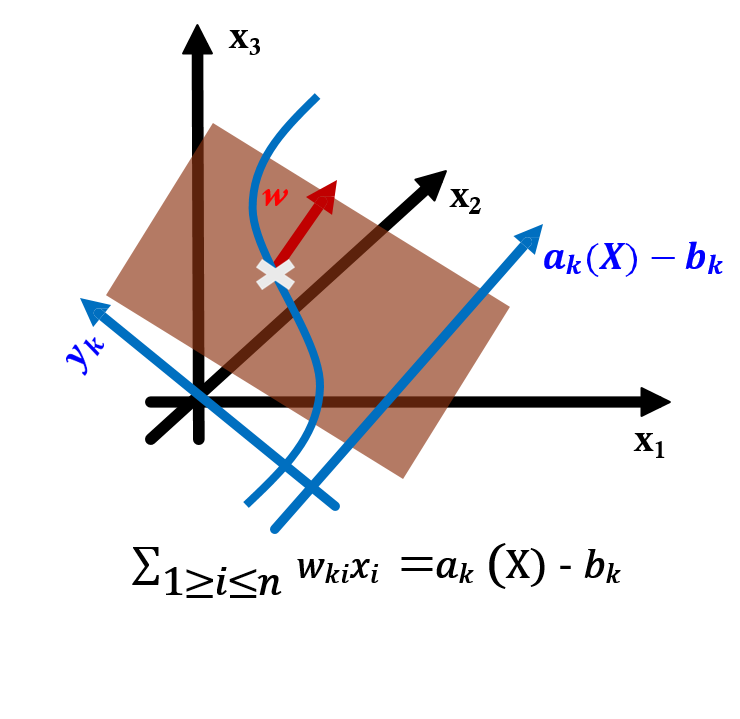
\includegraphics[scale=0.5]{fig14_5.png} 
\caption{logistic regression의 Activation function 적용 예시}
\label{fig:14-5}
\end{figure}
위의 그림은 logistic regression을 Output activation function으로서 적용한 결과를 graphical하게 보여주는 예시이다. 그림에서 hyperplane은 $W^{T}X+b=0$을 의미하는 평면으로서 hyperplane을 기준으로 전체 공간이 2개의 영역으로 나뉘어짐을 볼 수 있다. 이에 대해 logistic function이 hyperplane에 sharply adapt하고 있음을 확인할 수 있다. 
\subsection{Detour : Logistic function}

* Logistic function
\begin{equation}
g(x) = \frac{1}{1+e^{-x}}
\end{equation}
Logistic function은 대표적인 Sigmoid function의 예시이다. 그렇다면 Sigmoid function은 정확히 무엇을 의미하는 function일까? 아래의 특성을 만족하는 함수를 Sigmoid function이라고 칭한다.

* Sigmoid function
\begin{center}
    Bounded (유계성을 가진다.)\\
    Differentiable (모든 영역에서 미분가능하다.)\\
    Real function (실수 영역에서 정의되는 함수이다.)\\
    Defined for all real inputs (실수값을 가진 모든 input에 의해 정의가능하다.)\\
    with positive derivative (미분값이 양의 값을 가진다.)
\end{center}
\begin{figure}[ht] \centering 
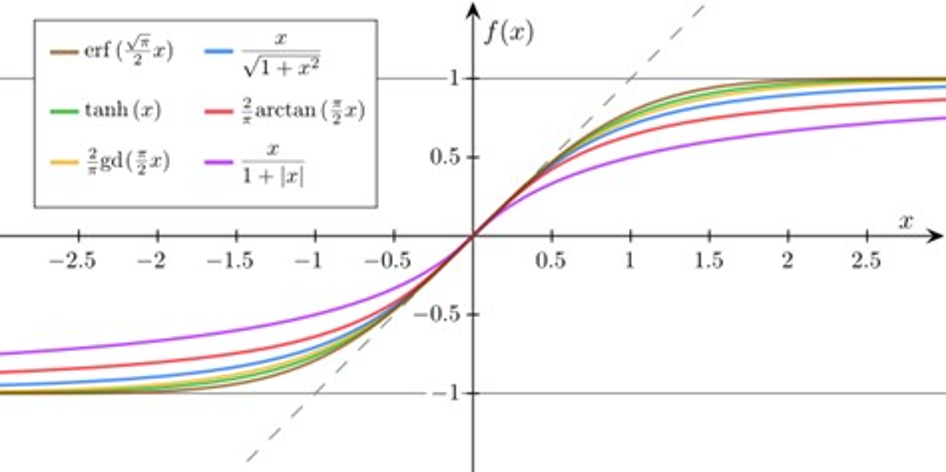
\includegraphics[scale=0.6]{fig14_6.png} 
\caption{다양한 Sigmoid function의 예시}
\label{fig:14-6}
\end{figure}
위의 그림과 같이 이러한 특성을 만족하는 sigmoid function은 매우 다양하다.  그 중에서도 Logistic function이 sigmoid function으로 자주 사용되는 이유는 무엇일까? 그 이유는 logistic function의 derivatve가 매우 계산하기 편리한 형태로 나오기 때문이다. 아래의 식을 보자.
\begin{eqnarray}
f(x) & = &  \frac{1}{1+e^{-x}} = \frac{e^{x}}{1+e^{x}}\\ 
\frac{d}{dx}f(x) & = & \frac{e^{x}(1+e^{x})-e^{x}e^{x}}{(1+e^{x})^{2}}\\
\frac{d}{dx}f(x) & = & \frac{e^{x}}{(1+e^{x})^{2}} = f(x)(1-f(x))
\end{eqnarray}
이처럼 미분한 결과가 원래 함수에 의한 형태로 나오기 때문에 복잡한 식의 계산시에 더 효율적으로 미분값을 구할 수 있다는 장점을 가지고 있다.
\subsection{Hyperbolic Tangent Function and Rectified Linear Function}
%-----------------------------------------------------------------
이번에는 Output Activation function으로 자주 이용되는 Hyperbolic tangent Function과 Rectified linear function에 대해 알아보겠다. 먼저 Hyperbolic Tangent function은 Logistic function과 달리 결과값의 범위가 -1부터 1로 정의된다. 이는 Logistic function이 가지고 있는 0과 1사이의 범위는 아니기 때문에 해당값을 확률 domain에 그대로 사용하기는 어려운 단점이 있다. 이외에도 Hyperbolic tangent Function은 모든 domain에 대한 derivative 값이 양수로 증가함수를 이루는 특징이 있는데, 해당 함수의 식을 아래와 같이 쓸 수 있다. \\

* Hyperbolic tangent function
\begin{equation}
g(x) = tanhx = \frac{sinhx}{coshx} = \frac{e^{x}-e^{-x}}{e^{x}+e^{-x}} = \frac{e^{2x}-1}{e^{2x}+1}
\label{eq:14-2-7}
\end{equation}
\begin{figure}[ht] \centering 
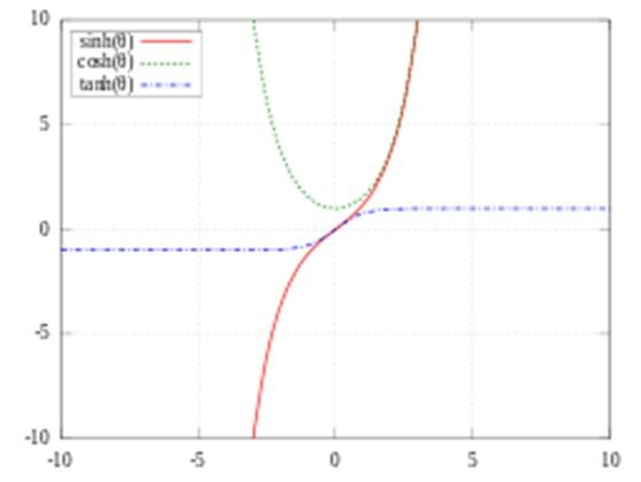
\includegraphics[scale=0.4]{fig14_7.png} 
\caption{Hyperbolic Tangent function}
\label{fig:14-7}
\end{figure}

다음은 Rectified linear activation function에 대해 알아보자. Rectified linear activation function의 경우 아래의 식에서 볼 수 있듯이 x값과 0중 더 큰 값을 함수로서 취하는 형태인데, 이에 따라 x가 0보다 작을 때는 0의 값을, 0보다 크거나 같은 경우에는 x 그 자체의 값을 가지게 된다. 이에 따라 x=0에서 미분불가능한 지점이 생겨나게 되는데, 이는 함수를 이용한 실제적인 계산을 수행하게 될 시 약점으로 작용할 수 있다. 

그럼에도 불구하고 본 함수가 자주 쓰이는 것은 Linear한 함수의 특징을 이용해 Regularization 시 sparse한 특성을 잘 반영시킬 수 있기 때문이다. 또한 S-curve를 이루는 다른 function과 달리 큰 값일수록 그 영향을 확실히 크게 받기 때문에 activation 각각에 대한 강조를 더 줄 수 있다는 장점도 있다. 

\begin{figure}[ht] \centering 
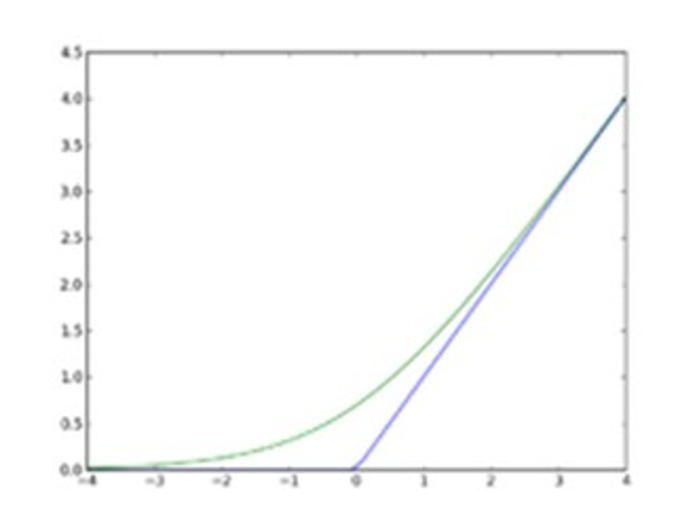
\includegraphics[scale=0.4]{fig14_8.png} 
\caption{Rectified Linear Function}
\label{fig:14-8}
\end{figure}

Rectified linear activation function의 x=0에서의 미분불가능을 smooth-out하기위해 만들어진 함수가 바로 Softplus function이다. softplus 함수는 모든 값에 대해 미분가능하면서도 derivative의 형태가 logistic function의 형태를 가진다는 점에서 계산의 용이성까지 가지고 있다.  \\

* Softplus function
\begin{equation}
g(x) = ln(1+e^{x}),  g^{'}(x)=\frac{1}{1+e^{-x}}
\label{eq:14-2-8}
\end{equation}

\subsection{Classification with Neuron}
%----------------------------------------------------------------
decision boundary가 정의된 Neuron들은 boundary를 기준으로 한 binary classification이 가능하다. 이에 대해 자세히 알아보도록 하겠다. 예를 들어 f(x) = $\frac{1}{1+e^{-x}}$라 하며 g(x) = $\theta$X라 할 경우 $P(Y|X)$ = f(g(x)) = $\frac{1}{1+e^{-x\theta}}$라고 할 수 있다. 즉 linear sum인 g(x)와 output activation function인 f(x)이 합성함수 형태가 되는 것이다. 

이를 그림으로 표현하면 아래와 같이 나타낼 수 있는데, decision boundary를 기준으로 output의 값에 따라 classification을 수행해주는 것을 확인할 수 있다. 이러한 linear decision boundary를 기준으로 classification을 할 경우 Logistic function의 분류 기준 값은 0.5, Hyperbolic tangent function의 기준값은 0이 될 것이다. 
\begin{figure}[ht] \centering 
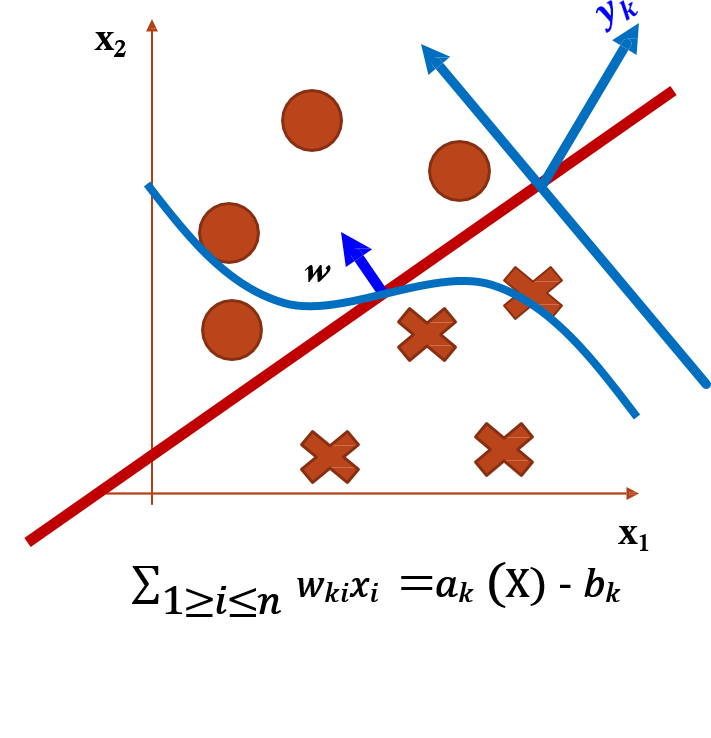
\includegraphics[scale=0.4]{fig14_9.png} 
\caption{인공 뉴런을 통한 분류 예시}
\label{fig:14-9}
\end{figure}
이처럼 Linear decision boundary가 존재하는 Classification의 경우 단일 인공뉴런을 통해서도 얼마든지 분류를 성공적으로 수행할 수 있다. 
\subsection{Problem of Linear Decision Boundary}
%----------------------------------------------------------------
아래의 그림은 위의 장의 분류 문제에 새로운 데이터가 추가된 상황을 나타낸 것이다. 이러한 상태로 각각의 데이터가 존재할 경우 Linear decision boundary로는 완벽한 분류가 불가능하다. 실제 현실에서는 아래와 같이 non-linear한 decision boundary가 필요한 case가 많은데, 이러한 문제를 해결하기 위해 하나의 decision boundary가 아닌 여러 개의 decision boundary를 중첩시키거나 조합하는 방식을 제안할 수 있다. 즉 여러 개의 neuron을 조합하여 문제를 해결하는 것이다. 
\begin{figure}[ht] \centering 
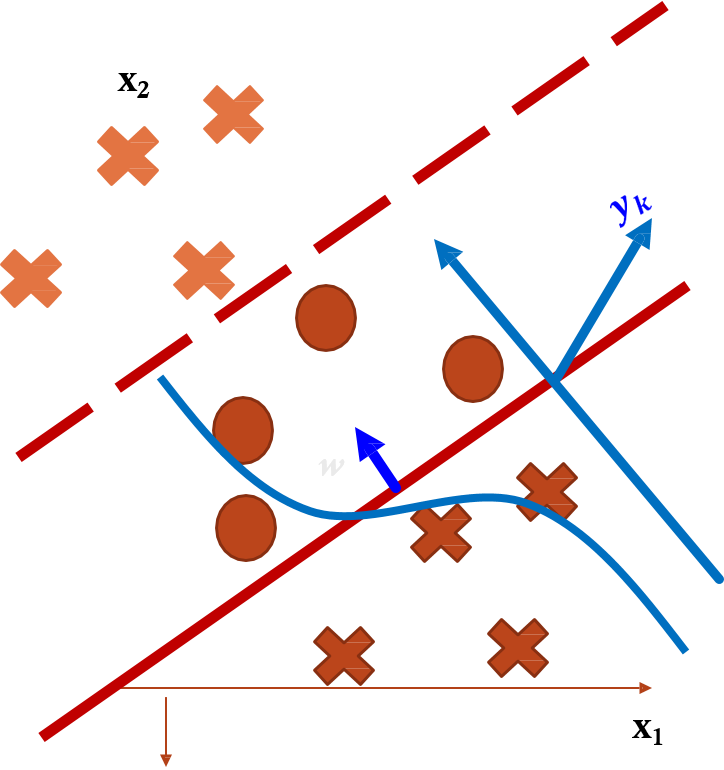
\includegraphics[scale=0.4]{fig14_10.png} 
\caption{Linear Decision Boundary로 분류가 불가능한 상황 예시}
\label{fig:14-10}
\end{figure}
\newpage
\subsection{Linear Boundary and Logic Operator}
boundary가 non-linear한 상황으로 자주 쓰이는 예시가 바로 XOR case이다. XOR case는 각각의 신호값이 서로 같을 때(ex : $x_{1}$ = 0,$x_{2}$ = 0)와 다를 때((ex : $x_{1}$ = 0,$x_{2}$ = 1) 결과값을 다르게 주는 방식인데, 아래의 그림을 통해 이를 직관적으로 확인할 수 있다.
\begin{figure}[ht] \centering 
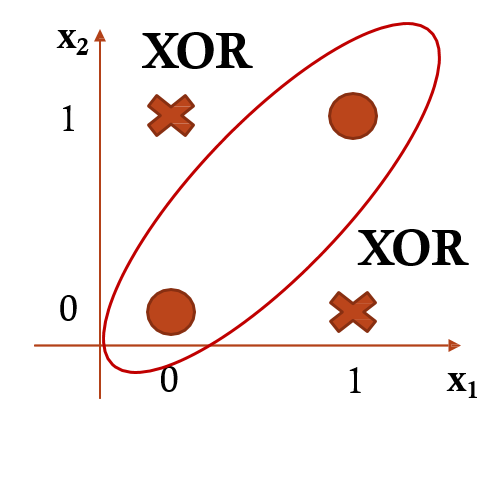
\includegraphics[scale=0.5]{fig14_11.png} 
\caption{XOR($x_{1}$,$x_{2}$) case}
\label{fig:14-11}
\end{figure}
위 그림의 X,O에 대해 1개의 decision boundary만으로는 완벽한 분류가 불가능하다. 이를 해결하기 위해 linear decision boundary를 각각의 경계에 1개씩, 총 2개를 배치할 경우 완벽한 분류가 가능해진다. 
\begin{figure}[ht] \centering 
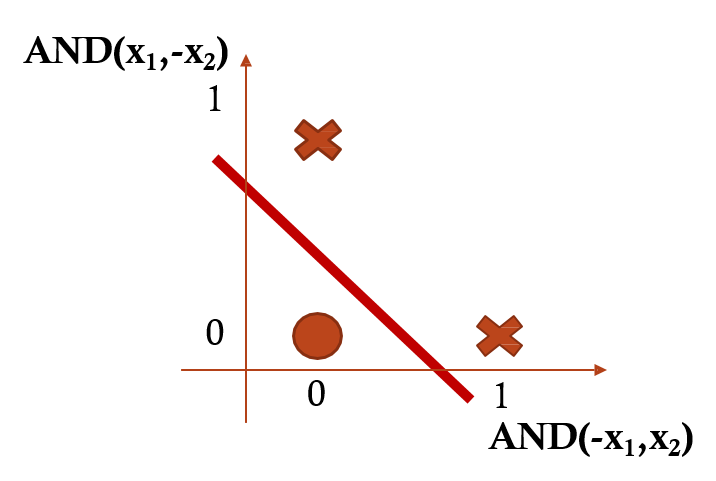
\includegraphics[scale=0.5]{fig14_12.png} 
\caption{AND(x,-y) OR AND(-x,y) case}
\label{fig:14-12}
\end{figure}\\
위의 그림은 AND에 의해 나타난 결과값들을 표현한 것이다. 각각의 case는 하나의 Decision boundary로 손쉽게 분류가 가능하다. 또한, 여러 AND case가 결합된 경우도 하나의 Decision boundary로 이를 해결할 수 있는데, 이러한 각각의 Decision boundary를 조합하여 XOR과 같은 복잡한 case 또한 분류가 가능해지는 것이다. decision boundary를 여러 개 중첩시킨다는 것은 결국 여러 개의 neuron을 조합한다는 의미이기도 하다. 이렇듯 단일 인공 뉴런이 아닌 여러 인공 뉴런들을 조합한 네트워크형 구조를 인공신경망 (Artificial neural network)이라고 한다.
\begin{figure}[ht] \centering 
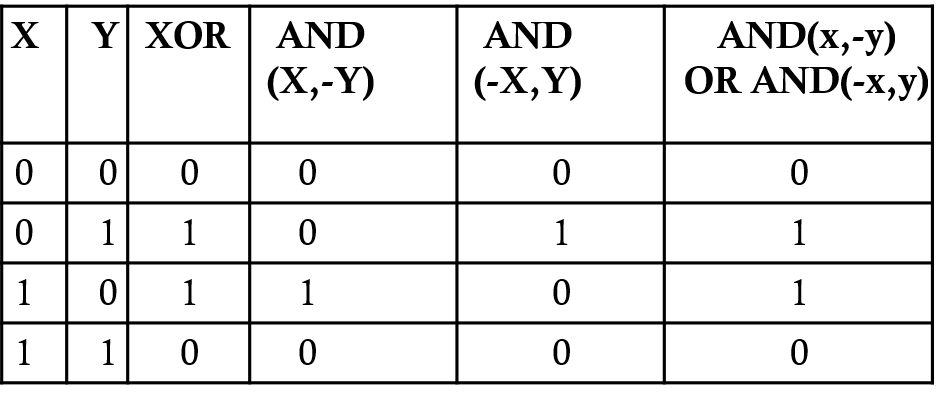
\includegraphics[scale=0.5]{fig14_13.png} 
\caption{x,y의 값 변화에 따른 각 case의 operation 결과}
\label{fig:14-13}
\end{figure}

\section{Artificial Neural Network}
%----------------------------------------------------------------
\subsection{Artificial Neural Network}
%----------------------------------------------------------------
아래의 그림은 linear decision boundary의 한계를 극복하기 위해 제안된 인공신경망 (Artificial neural network)의 예시이다. Layer는 각각 input layer, hidden layer, Output layer로 구성되며 Layer 각각이 가진 원안에 들어가는 것이 single perceptron (artificial neuron)인 것이다. 아래의 그림의 경우 7개의 neuron으로 구성된 신경망이라 할 수 있다. 
\begin{figure}[ht] \centering 
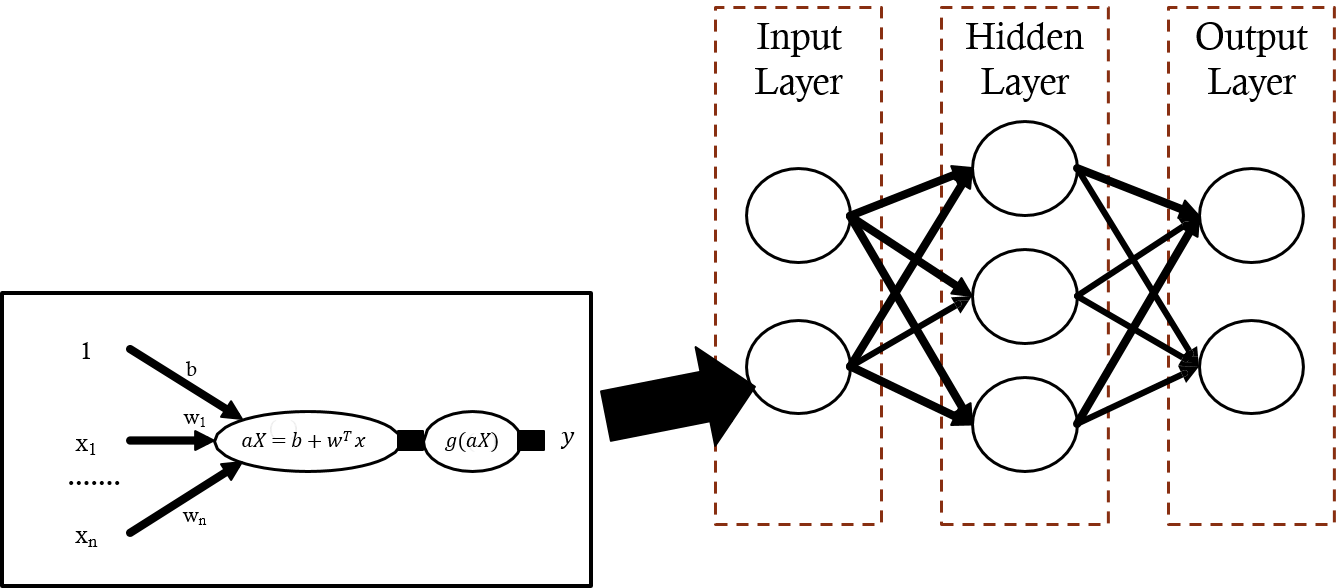
\includegraphics[scale=0.5]{fig14_14.png} 
\caption{인공신경망 (Artificial neural network) 예시}
\label{fig:14-14}
\end{figure}
또한 동일한 layer에 위치한 각 neuron들은 서로 connection이나 interaction을 이루지 않는다. 각 layer의 전후에 있는 layer와 연결관계를 가지고 있으며 이를 통해 interaction이 이루어지는 형태인 것이다. 

위와 같이 input layer의 정보가 output layer까지 순차적으로 흐를 수 있도록 구성된 인공신경망을 Feed-forward neural network라고 한다. 각각의 layer는 data를 입력해주는 단계인 input layer와 그에 따른 최종 결과물을 출력해주는 output layer, 그 사이에 존재하는 Hidden layer로 구성되는데, 최근의 deep neural network의 경우 Hidden layer의 개수를 많도록 한 인공신경망을 의미한다. 
\subsection{Effect of Multiple Perceptron}
%----------------------------------------------------------------
아래의 그림과 같이 3개의 neuron (perceptron)을 활용하여 간단한 인공신경망을 만들어보았다. 즉, single input layer에 2개의 perceptron, single output layer에 1개의 perceptron이 배치된 형태라고 할 수 있다. 
\begin{figure}[ht] \centering 
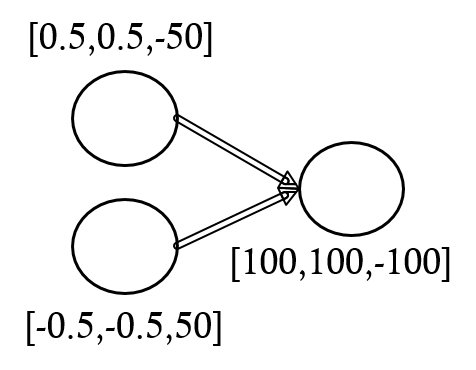
\includegraphics[scale=0.5]{fig14_15.png} 
\caption{neuron 관점에서 표현한 single input layer와 single output layer를 가진 인공신경망 예시}
\label{fig:14-15}
\end{figure}
이러한 인공신경망 예시를 통해 만들어낸 결과를 아래와 같이 표현할 수 있는데, 각각의 single perceptron이 만들어낸 결과가 x1, x2에 대하여 각각 h1, h2와 같이 linear하게 표현된다면 이들을 조합하여 만들어낸 최종 Output인 $O_{1}$의 경우 x1과 x2에 대하여 non-linear한 관계를 띔을 알 수 있다. 즉, 여러 개의 perceptron이 조합되면서 non-linear한 관계에 대한 정의 또한 가능해진 것이다. 
\begin{figure}[ht] \centering 
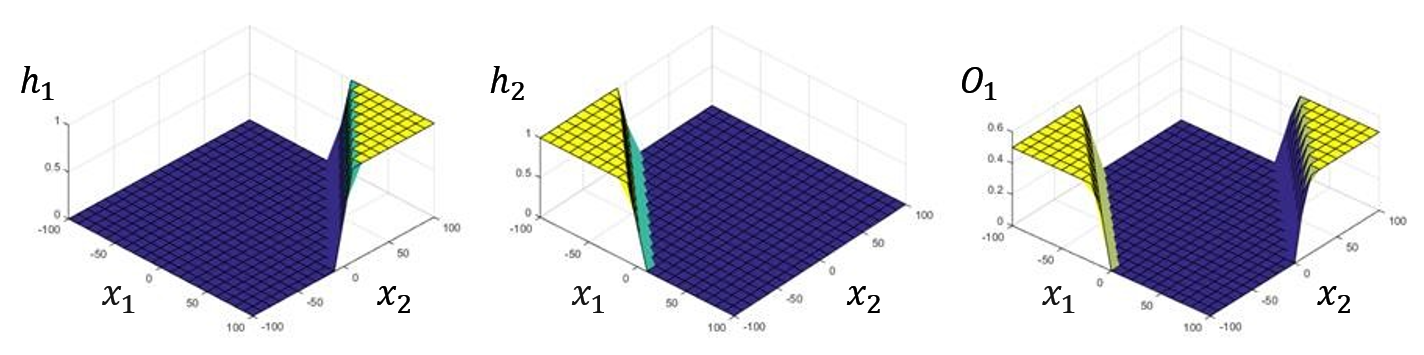
\includegraphics[scale=0.5]{fig14_16.png} 
\caption{하나의 인공 뉴런이 만들어낸 결과 (좌, 중간)와 이들을 조합한 결과 (우)}
\label{fig:14-16}
\end{figure}
\newpage
\subsection{Linking Multiple Neurons}
아래의 그림은 각각 neuron 관점과 data 관점에서 표현된 인공신경망의 예시이다. 아래와 같이 인공신경망은 data, neuron 각각의 관점에서 자유롭게 표현이 가능하다. 그렇다면 Hideen layer를 지닌 neural network의 정보 전달 식은 어떻게 표현할 수 있을까?\\
\begin{figure}[ht] \centering 
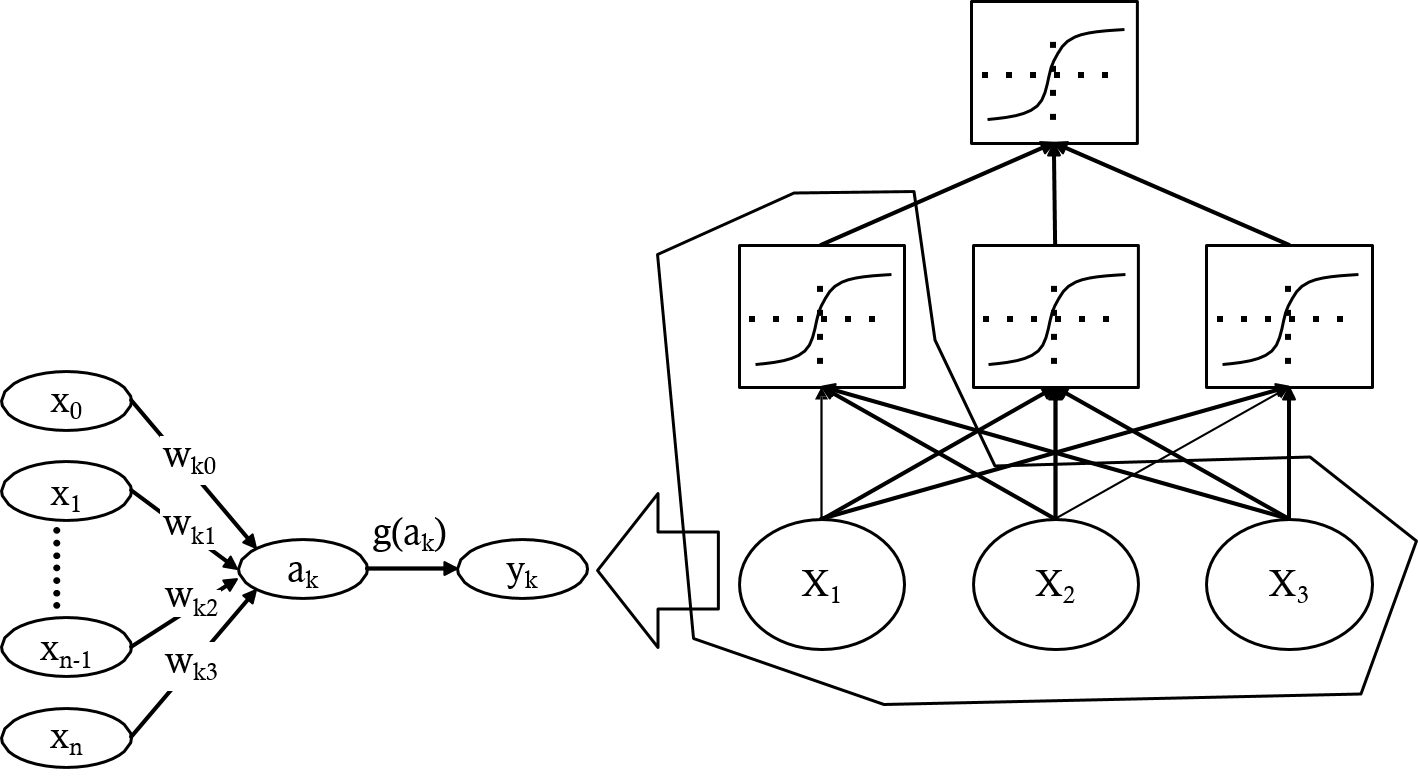
\includegraphics[scale=0.5]{fig14_17.png} 
\caption{neuron 관점에서 표현한 인공신경망 (좌)과 data 관점에서 표현한 인공신경망 (우)}
\label{fig:14-17}
\end{figure}
* Hidden layer neuron input activation function
\begin{equation}
a(X) = b + W^{1}_{i,j}X
\label{eq:14-2-9}
\end{equation}
먼저 hidden layer의 input activation의 경우 위와 같이 각 x의 weight에 대한 linear sum을 구한 다음 biased term인 b를 이에 추가하는 방식으로 이뤄진다.\\
* Hidden layer neuron output activation function
\begin{equation}
h(X) = g(a(X))
\label{eq:14-2-10}
\end{equation}
hidden layer의 output activation은 linear sum 형태로 구한 a(X)를 output activation function인 g를 통해 변환함으로써 실행된다. \\
* output layer neuron output activation function
\begin{equation}
f(X) =o(b + wh(X))
\label{eq:14-2-11}
\end{equation}
각 hidden layer에 대한 연산이 모두 종료된 후에는 최종적으로 output layer에 대한 activation을 실행해주며 이에 대한 식은 위와 같다. 
\subsection{Output activation function}
neural network를 이용하여 0,1과 같은 binary classification을 한다고 하자. 이 경우 Logistic function, Relu function와 같은 sigmoid function이 효과적으로 사용될 수 있다. 허나, binary가 아닌 여러 개의 choice에 대한 classification 문제는 sigmoid function으로 해결하기가 쉽지 않다.

이러한 문제를 해결해주는 대표적인 activation function이 바로 softmax activation function이다.\\

* softmax function
\begin{equation}
o(a) = softmax(a) = [\frac{exp(a_{1})}{\sum_{c}exp(a_{c})},...,\frac{exp(a_{c})}{\sum_{c}exp(a_{c})}]
\label{eq:14-2-12}
\end{equation}
C개의 class를 갖는 상황에서 softmax function은 위와 같은 식을 가지게 되며 exponential을 취해줌에 따라 각 dimension의 값이 모두 positive하다. 또한 exponential에 의해 각 값의 차이가 비교적 크게 나타나는데, 이를 통해 decision boundary에 대한 adaptation을 매우 sharp하게 가져올 수 있다. 또한 normalized 된 값을 사용하기에 각 값의 sum(합)을 1이 되며 이는 확률변수로서의 모델링에 매우 적절한 형태르 지닌다고 볼 수 있다.
\subsection{Multiple Layers of Neural Network}
L개의 hidden layer를 지닌 인공신경망을 생각해보자. 각각의 layer 및 neuron을 이어주는 weight term과 biased term은 어느 layer 사이에 있냐에 따라 다른 값을 가질 것이다. 이러한 구조를 아래의 그림처럼 표현할 수 있다.
\begin{figure}[ht] \centering 
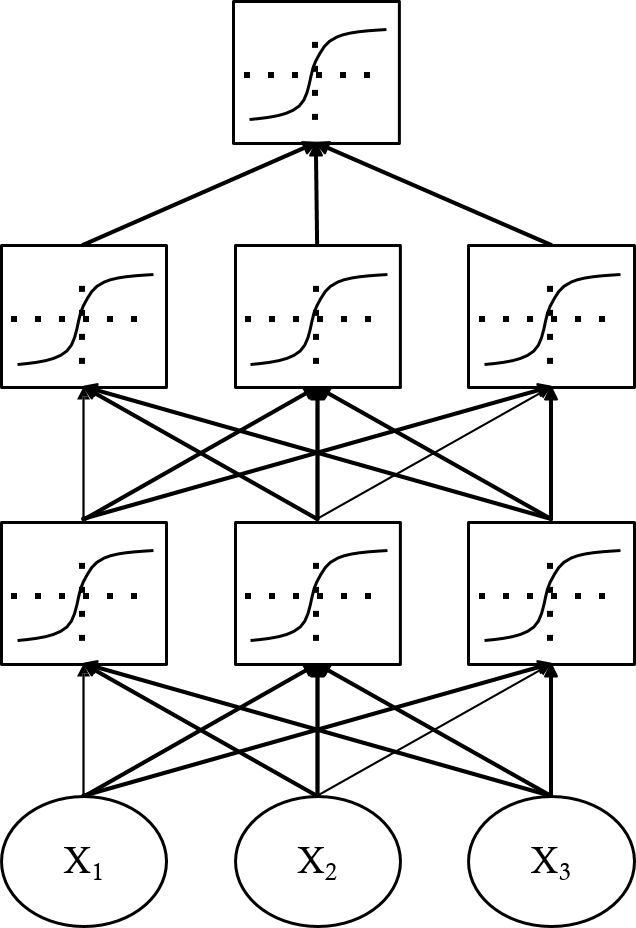
\includegraphics[scale=0.5]{fig14_19.png} 
\caption{data 입장에서 표현한 Multiple layer를 지닌 인공신경망 예시}
\label{fig:14-18}
\end{figure}
위의 식에 대해 k번째 (hidden) layer의 neuron에 대한 표현을 $h^{(k)}$이라고 하자. 각 layer간 connection의 역할을 하는 weight (W)와 biased term (b)을 고려하여 식을 써주면 아래와 같이 나타낼 수 있다. 또한 각 layer의 output activation function으로는 sigmoid function, softmax function과 같은 다양한 함수를 각 상황에 맞게 선택적으로 사용할 수 있다. \\

* neuron input activation function for the k-th layer
\begin{equation}
a^{k}(x) = b^{k} + W^{k}h^{(k-1)}(x)
\label{eq:14-2-13}
\end{equation}

* neuron output activation function for the k-th layer
\begin{equation}
h^{k}(x) = g(a^{k}(x))
\label{eq:14-2-14}
\end{equation}

* output layer activation
\begin{equation}
h^{L+1}(x) = o(a^{L+1}(x)) = f(x)
\label{eq:14-2-15}
\end{equation}
\section{Training neural network}
위의 장을 통해 인공신경망 (artificial neural network)의 구조를 알아보았다. 이제 이러한 구조를 통해 데이터를 학습시키는 방법에 대해 알아보도록 하겠다. Learning, 즉 Training은 결국 parameter를 inference하는 과정이며 이는 주어진 data에 기반하여 모델의 loss term, likelihood 등을 optimize하는 과정이라 할 수 있다. optimization의 방식으로 gradient descent method, quadratic method 등 다양한 방법이 제시되었는데, neural network model의 경우 어떤 방법을 통해 training을 진행하는 지 함께 알아볼 것이다.
\subsection{Derivative of Activation function}
%----------------------------------------------------------------
logistic function을 output activation function으로 하는 neuron에 대한 activation 과정을 f(g(x))으로 표현할 때 각각의 f(x)와 g(x)를 우리는 아래와 같이 쓸 수 있었다. 
\begin{center}
    f(x) = $\frac{1}{1+e^{-x}}$\\
    g(x) = WX + b
\end{center}
즉, f(x)는 output activation function을 의미하며 g(x)는 input에 대하여 각각의 weight 및 biased term을 고려한 linear sum 형태가 되는 것이다. 이를 학습시킨다는 것은 결국 weight와 biased term을 학습시킨다는 것으로 이해할 수 있다. \\

* derivative of Logistic function ($\frac{1}{1+e^{-x}}$)
\begin{eqnarray}
f(x) & = &  \frac{1}{1+e^{-x}} = \frac{e^{x}}{1+e^{x}}\\ 
\frac{d}{dx}f(x) & = & \frac{e^{x}(1+e^{x})-e^{x}e^{x}}{(1+e^{x})^{2}}\\
\frac{d}{dx}f(x) & = & \frac{e^{x}}{(1+e^{x})^{2}} = f(x)(1-f(x))
\end{eqnarray}
앞의 장을 통해 logistic function은 함수의 derivative가 원래 함수 f(x)에 의해 위와 같이 표현가능하다는 점을 밝혔다. 이는 mathematical notation에 있어 매우 편리한 특성을 지니는데, 다른 activaton function들 또한 비슷한 특성을 지니고 있다.\\

* derivative of hyperbolic tangent function
\begin{eqnarray}
f(x) & = &  tanh(x) = \frac{e^{2x}-1}{e^{2x}+1}\\
\frac{d}{dx}f(x) & = & 1 - f^{2}(x)
\end{eqnarray}
위의 식과 같이 hyperbolic tangent function 또한 derivative가 본래 함수 f(x)에 의해 표현가능함을 알 수 있다. \\

* derivative of Relu\\
Relu의 경우 x=0에서 미분불가능하다. x=0보다 큰 지점의 gradient와 x=0보다 작은 지점의 gradient 값이 서로 다르기 떄문이다. 이를 해결하기 위해 relu의 경우 sub-gradient method를 이용하여 derivative를 구한다.
\begin{equation}
f(x) - f(x_{0}) \geq c(x-x_{0}) \; \rightarrow \; c \in  \;\;\mid lim_{x \rightarrow x^{-}_{o}}\frac{f(x)-f(x_{0})}{x-x_{0}}, lim_{x \rightarrow x^{+}_{o}}\frac{f(x)-f(x_{0})}{x-x_{0}} \mid \nonumber
\end{equation}
relu의 경우 x=0에서 미분불가능하기 때문에 0을  기점으로 $0^{-}$와 $0^{+}$에 대한 gradient를 구하면 각각 0과 1의 값을 가지게 된다. 이에 대해 실제 derivative값은 0과 1사이에서 임의의 값을 택하는 방식으로 정하게 된다. 이를 통해 derivative c에 대한 값을 각각의 case에 맞게 적절히 정할 수 있다. 

\subsection{Sample Neural Network}
%----------------------------------------------------------------
이번 장에서는 임의의 sample Neural network를 통해 실제 학습 및 parameter의 inference가 어떻게 이루어지는 지 알아보도록 하겠다. 아래의 그림은 두 개의 hidden layer를 가진 neural network이다. 

\begin{figure}[ht] \centering 
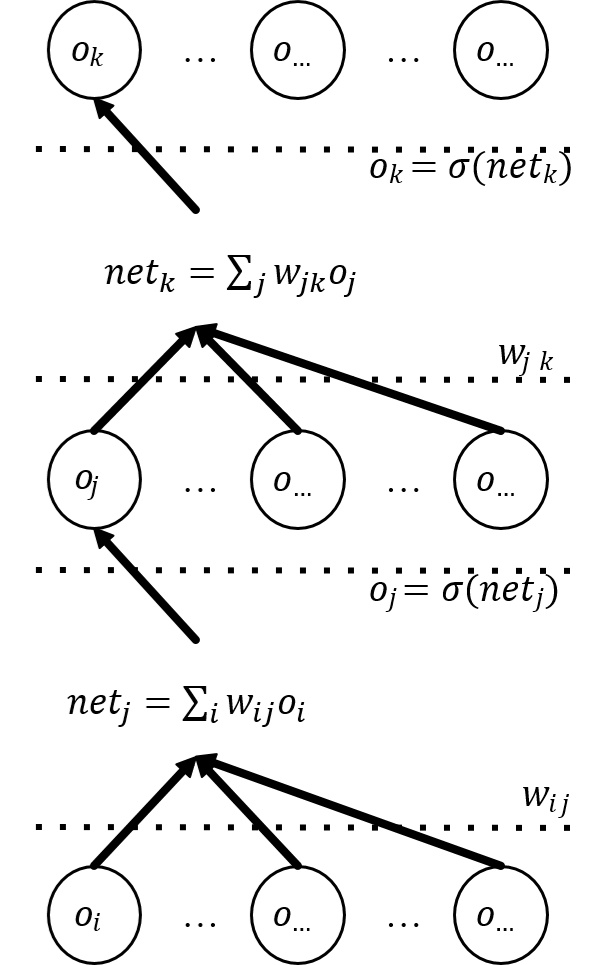
\includegraphics[scale=0.5]{fig14_20.png} 
\caption{data 관점에서 나타낸 두 개의 hidden layer를 가진 neural network}
\label{fig:14-19}
\end{figure}

위의 그림은 data의 관점에서 neural network의 흐름을 나타내어 보았는데, 각각의 data layer는 하나의 neuron layer를 거침으로써 새로운 data layer에 다다르게 되며 각각을 이어주는 매개체 역할을 하는 것이 data layer와 neuron layer를 이어주는 weight와 biased term이 될 것이다. 

또한 각각의 hidden neuron layer에서 weight와의 linear sum으로 표현되는 input activation 과정을 아래와 같이 쓸 수 있다. 
\begin{equation}
net_{k} = \sum_{j}w_{jk}o_{j},\;\; net_{j} = \sum_{i}w_{ij}o_{i}
\end{equation}
그 다음, input activation 과정을 거친 $net_{j}$와 $net_{k}$을 output  activation function을 통해 변환시켜줘야 한다. output activation function으로 logistic function을 택했다고 하자. \\
* derivative of logistic function 
\begin{eqnarray}
f(x) & = &  \frac{1}{1+e^{-x}} = \frac{e^{x}}{1+e^{x}}\\ 
\frac{d}{dx}f(x) & = & \frac{e^{x}(1+e^{x})-e^{x}e^{x}}{(1+e^{x})^{2}}\\
\frac{d}{dx}f(x) & = & \frac{e^{x}}{(1+e^{x})^{2}} = f(x)(1-f(x))
\end{eqnarray}
logistic function은 derivative의 형태를 위와 같이 나타낼 수 있는 성질이 있었다. 이를 이용하여 output activation을 진행할 경우 아래와 같이 식을 쓸 수 있다. \\
* output activation
\begin{eqnarray}
\frac{d}{dx}\sigma(net_{j}) & = &  \sigma(net_{j})(1-\sigma(net_{j}))\\
&=& o_{j}(1-o_{j})
\end{eqnarray}
위의 과정을 통해 neural network의 data가 어떤 방식으로 전달되고 변환되는 지를 이해해보았다. 이러한 체계를 가진 neural network를 제대로 활용하기 위해서는 특정한 목표 혹은 목적을 가지고 parameter를 inference해주고 learning하는 과정이 필요하다. 이를 위해서는 최적화의 주체가 되는 목적식이 필요한데, 목적식 (loss function)을 아래와 같이 정의하고자 한다.\\
* Definition of loss function
\begin{equation}
E = \frac{1}{2}(\sum_{k}(t_{k}-o_{k})^{2})
\end{equation}
위의 식에서 $t_{k}$는 우리가 neural network에 주고자하는 supervision (지도)값이 될 것이고 $o_{k}$의 경우 예측을 통해 만들어진 prediction output이 될 것이다. 즉 지도값과 예측값간의 차이를 minimize하는 방향으로 neural network의 parameter를 학습시키겠다는 것이다. 이러한 parameter는 neural network의  weight를 나타내는 $w_{ij}$, $w_{jk}$가 될 것이다. \\
Weight의 학습을 위해서는 weight에 대한 목적식의 gradient, 즉 $\frac{\partial E}{\partial w_{ij}}$,$\frac{\partial E}{\partial w_{jk}}$를 알아내야 할 것이다. 허나 각각의 식들이 weight parameter와 직접적으로 연관되지 않은 경우도 있기에 각각의 layer를 잇는 chain rule을 통해 학습을 진행해야 한다.

\subsection{Learning Single Depth}
%----------------------------------------------------------------
\begin{equation}
E = \frac{1}{2}(\sum_{k}(t_{k}-o_{k})^{2})
\end{equation}
error term을 minimize하기 위해서는 이에 대한 weight의 gradient 계산이 필요하다는 것을 알 수 있었다. 즉 각각의 layer마다 정의된 weight 별로 gradient를 구하는 작업이 필요한데, 먼저 두개의 layer 중 output에 더 가까운 layer의 weight에 해당하는 $w_{jk}$에 대한 gradient를 구해보도록 하겠다. 
\begin{eqnarray}
\frac{\partial E}{\partial w_{jk}} & = &  \frac{\partial E}{\partial o_{k}}\frac{\partial o_{k} }{\partial net_{k}}\frac{\partial net_{k} }{\partial w_{jk}}\\ 
& = & -(t_{k}-o_{k})o_{k}(1-o_{k})o_{j}
\end{eqnarray}
Error term과 weight는 서로 연관관계가 있지만 식에서 직접적으로 weight가 정의되지 않았기 때문에 chain rule을 통해 gradient를 구해야한다. 이를 위해 $o_{k}$, $net_{k}$, $w_{jk}$에 대한 gradient를 차례대로 구함으로써 chain rule을 적용할 수 있다. \\
그 결과 $\frac{\partial E}{\partial o_{k}}$의 값은  $-(t_{k}-o_{k})$이 된다. 또한, $\frac{\partial o_{k}}{\partial net_{k}}$은 결국 output activation function에 대한 derivative의 형태를 띄므로  $o_{k}(1-o_{k})$이 되며 $\frac{\partial net_{k} }{\partial w_{jk}}$의 경우 $o_{j}$이 된다.\\
gradient를 구한 다음, 이미 배운 바 있는 gradient descent method를 통해 weight를 학습시킬 수 있다. 그 과정에서 Delta signal이라는 notation을 도입하고자 한다. Delta signal은 error term에 대한 weight의 derivative에서 위의 layer 정보에 의해 내려오는 값인 $(t_{k}-o_{k})$과 $o_{k}(1-o_{k})$의 곱으로 이루어져 있다. \\

* Delta signal 
\begin{equation}
\delta_{k} = (t_{k}-o_{k})o_{k}(1-o_{k})
\end{equation}
* Gradient descent method applied on neural network learning ($\eta$ is the learning rate)
\begin{eqnarray}
w^{t+1}_{jk} & \leftarrow &  w^{t}_{jk} - \eta\frac{\partial E}{\partial w_{jk}}\\
& = & w^{t}_{jk} - \eta(-(t_{k}-o_{k})o_{k}(1-o_{k})o_{j})\\
& = & w^{t}_{jk} - \eta(-\delta_{k}o_{j}) = w^{t+1}_{jk} + \eta\delta_{k}o_{j}
\end{eqnarray}
위와 같이 각각의 iteration마다 weight는 $\eta$값을 learning rate로 사용하여 점차 error term을 minimize하는 방향으로 값을 변화해간다. 또한, weight를 learning해나갈 때 각각에 대한 값의 변화는 learning rate, delta signal, 해당 data 값의 곱과 같아지는데, 이를 나타내어주는 식이 바로 delta rule이다.\\

* delta rule
\begin{equation}
\Delta w_{jk} = \eta\delta_{k}o_{j}=\eta(t_{k}-y_{k})\sigma^{'}(h_{k})x_{j}
\end{equation}

\subsection{Learning Two Depth}
%----------------------------------------------------------------
앞의 장을 통해 single depth의 layer에서 weight 학습 방식에 대해 알아보았다. 이번에는 two depth를 가진 layer에 대한 weight의 학습 방식에 대해 알아보도록 하겠다. 

\begin{figure}[ht] \centering 
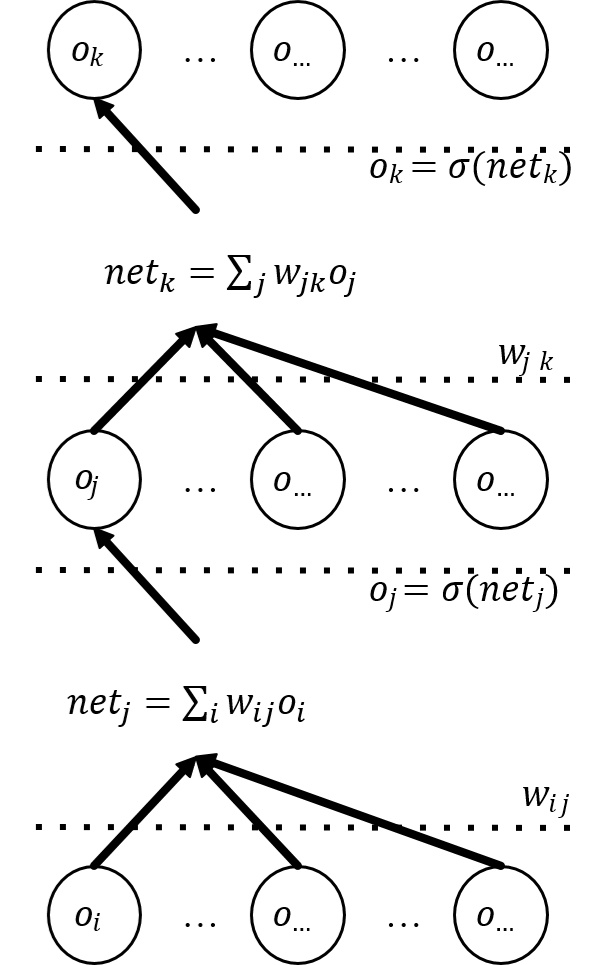
\includegraphics[scale=0.5]{fig14_20.png} 
\caption{data 관점에서 나타낸 두 개의 hidden layer를 가진 neural network}
\label{fig:14-20}
\end{figure}

* Loss function
\begin{equation}
E = \frac{1}{2}(\sum_{k}(t_{k}-o_{k})^{2})
\end{equation}
single depth의 경우 $w_{jk}$이 학습의 주체였으며 loss function에 대한 $w_{jk}$의 gradient 값 중 layer의 윗부분에서 내려받는 값을 delta signal이라 정의하여 아래와 같이 나타낼 수 있었다.\\
만약 여러 개의 층을 이룬 layer에 대한 weight에 대해서도 같은 방식으로 학습을 시킬 수 있다면 신경망의 윗부분에 대한 정보, 즉 위에서 정의한 delta signal을 활용하여 보다 간단한 형식으로 학습이 가능할 것이다. \\
* Delta signal
\begin{equation}
\delta_{k} = (t_{k}-o_{k})o_{k}(1-o_{k})
\end{equation}
이제 two-depth layer에서 아래쪽 layer의 weight에 해당하는 $w_{ij}$에 대한 학습을 알아보도록 하겠다. 아래의 식은 loss function (E)에 대한 $w_{ij}$의 gradient를 구하는 식이다.
\begin{eqnarray}
\frac{\partial E}{\partial w_{ij}} & = &  \sum_{k}\frac{\partial E}{\partial o_{k}}\frac{\partial o_{k} }{\partial net_{k}}\frac{\partial net_{k} }{\partial o_{j}}\frac{\partial o_{j}}{\partial net_{j}}\frac{\partial net_{j} }{\partial w_{ij}}\\ 
& = & \sum_{k}-(t_{k}-o_{k})o_{k}(1-o_{k})\frac{\partial net_{k} }{\partial o_{j}}\frac{\partial o_{j}}{\partial net_{j}}\frac{\partial net_{j} }{\partial w_{ij}}\\
& = & \sum_{k}-\delta_{k}w_{jk} \times o_{j}(1-o_{j}) \times o_{i}\\
& = & -o_{i}o_{j}(1-o_{j}) \sum_{k}\delta_{k}w_{jk}
\end{eqnarray}
$\frac{\partial E}{\partial w_{jk}}$와 달리 $\frac{\partial E}{\partial w_{ij}}$의 식에서는 k에 대한 summation이 이루어진 것을 알 수 있다. 이렇듯 식 상에서 차이가 나는 이유는, $w_{jk}$의 경우 output activation의 결과물인 수많은 $o_{k}$ (k=1,2,3...,K) 중 특정 k번째 output에만 영향을 미치지만 $w_{ij}$은 중간의 data layer에 대한 output activation의 결과값인 $o_{j}$가 k개의 모든 output에 영향을 미치기 때문이다. 고로 k개의 output ($o_{k}$) 전부에 대한 loss function을 고려해줘야하는 것이다. \\
$\frac{\partial E}{\partial w_{jk}}$와 마찬가지로 $\frac{\partial E}{\partial w_{ij}}$ 또한 chain rule을 이용하여 각각에 대한 gradient를 순차적으로 구해나간다. 이 과정에서 미리 정의해둔 delta signal을 활용하여 식을 더 간단히 나타낼 수 있다.\\
* Delta signal
\begin{equation}
\delta_{j} = o_{j}(1-o_{j})\sum_{k}\delta_{k}w_{jk}
\end{equation}
최종적으로 나타낸 식에서 $o_{i}$는 input으로 사용되는 data를 의미하며 $o_{j}(1-o_{j})$은 해당 layer의 output activation function  (logistic function)에 대한 derivative를 의미한다. 남은 부분인 $\sum_{k}\delta_{k}w_{jk}$은 윗 layer에서 넘겨받은 delta signal과 weight term을 의미한다. 결국 $\frac{\partial E}{\partial w_{ij}}$을 구하기 위해서는 해당 layer의 정보이외에 윗부분에서 정의된 delta signal과 weight term만 알면 되는 것이다. 이는, delta signal이 각각의 depth에 해당하는 layer마다 재귀적 (recursive)으로 정의됨으로써 weight에 대한 derivative 또한 재귀적으로 (recursive) 구할 수 있게 됨을 의미한다. 이 과정에서 정의되는 해당 layer의 delta signal 또한 위와 같이 정의할 수 있다. 신경망의 윗부분에서부터 delta signal을 차례대로 구해나간다면 각 layer마다의 delta signal 값을 재귀적으로 구할 수 있으며, 이를 통해 전체 신경망에 대한 weight의 학습이 가능해질 것이다. 이러한 방식의 학습 알고리즘을 Back-propagation algorithm이라고 한다. 이에 대한 내용은 다음 장에서 더 자세히 다루도록 할 것이다.
\begin{eqnarray}
w^{t+1}_{ij} & \leftarrow &  w^{t}_{ij} - \eta\frac{\partial E}{\partial w_{ij}}\\
& = & w^{t}_{ij} - \eta\frac{\partial E}{\partial w_{ij}}\\
& = & w^{t}_{ij} - \eta(-o_{i}\delta_{j}) = w^{t}_{ij} + \eta o_{i}\delta_{j}
\end{eqnarray}
위와 같이 $\frac{\partial E}{\partial w_{ij}}$을 구한 이후에는 gradient descaent method를 통해 weight term을 각 iteration마다 위와 같이 학습시켜 나간다. 

\subsection{Back-propagation}
%----------------------------------------------------------------
multiple depth를 가진 neural network의 각 layer에 대한 weight는 back -propagation을 통해 차례대로 학습할 수 있음을 배웠다. 아래는 이러한 back-propagation의 과정을 pseudo-code의 형태로 나타낸 것이다. \\

\textbf{* Back-propagation}
\begin{center}
\textbf{initialize} network's weight and \textbf{repeat}

\textbf{1) forward pass of the neural network}
\begin{center}
    $o_{k} = f(x;w)$\\
    $E = \frac{1}{2}(\sum_{k}(t_{k}-o_{k})^{2})$
\end{center}

\textbf{2) backward pass of the neural network}
\begin{center}
    Calculate $\delta_{k} = (t_{k}-o_{k})o_{k}(1-o_{k})$\\
    For the backward-pass from the top to the bottom, Calculate $\delta_{j} = o_{j}(1-o_{j})\sum_{k}\delta_{k}w_{jk}$
\end{center}

\textbf{3) weight update}
\begin{center}
    update $w_{jk}$ with $w^{t+1}_{jk} \leftarrow w^{t}_{jk} + \eta\delta_{k}o_{j}$\\
    For the backward-pass from the top to the bottom, Update $w^{t+1}_{ij} \leftarrow w^{t}_{ij} + \eta o_{i}\delta_{j}$
\end{center}
\textbf{Until all weights Converge}\\
\end{center}

인공신경망 내의 모든 weight에 대해 initialization을 거친 후, 먼저 input layer에서 output layer까지 data와 weight를 고려한 값을 순서대로 구해나간다. 이를 신경망의 forward-pass라고 하는데, 각각의 값들을 구해줌에 따라 신경망의 초기 error term (loss function)값 또한 나오게 될 것이다. 

그 다음, 각 layer 별로 구한 값에 대해 output layer부터 순서대로 delta signal($\delta$)을 재귀적으로 구해간다. two-depth의 상황에서는 $\delta_{k}$, $\delta_{j}$의 순서로 값을 구해갈 것이다. 이를 backward pass라고 표현한다. 

각각의 layer에 대한 delta signal의 계산을 완료한 이후에는 학습의 대상이 되는 weight를 update해주기만 하면 된다. 위의 과정은 모든 weight가 특정 값의 변화 미만으로 수렴(Converge)할 때까지 반복된다. 
\section{Concepts related to Neural networks}
%----------------------------------------------------------------
\subsection{Weight Initialization}
%----------------------------------------------------------------
인공신경망에서 학습의 주체가 되는 weight의 초기값을 잘 잡아주는 것은 매우 중요하다. 이러한 initialization이 모델의 정확도를 향상시키는 데 매우 큰 영향을 주기 때문이다. 이번 장에서는 weight 및 biased term의 initialization에 대해 알아보도록 하겠다.

biased term의 경우 단어의 의미가 내포하듯 초기 값을 0으로 잡아주어도 큰 문제가 없다. 중요한 건 weight term인데, 가령 biased term과 같이 weight term의 초기값을 0으로 잡아줄 경우 hyperbolic tangent function을 activation function으로 사용했을 때 각 weight의 gradient가 모두 0이 되는 등 saddle point로 갇힐 위험이 있다. 

마찬가지로 모든 weight term의 값을 특정 값으로 같게 만들어줄 경우 신경망의 randomness가 사라지고 모델의 symmetric한 특성 때문에 학습에 효율을 떨어뜨릴 수 있다. 

이러한 문제를 해결하기 위해 weight를 특정 영역의 distribution에서 sampling하는 방법을 제안할 수 있다. 아래의 경우 uniform distribution에 대하여 아래와 같이 정의된 영역에서 weight를 sampling하고있다. 
\begin{center}
* \textbf{Recipe} : sample $W^{k}_{i,j}$ from U[-b,b] where b = $\frac{\sqrt{6}}{\sqrt{H_{k}+H_{k}-1}}$\\
\end{center}
이러한 sampling을 통해 weight간의 symmetry를 방지함은 물론 0이 아닌 0 주변의 값으로 weight term을 각각 assign해줄 수 있다.
\subsection{Stochastic Gradient Descent}
%----------------------------------------------------------------
위의 장에서는 인공신경망의 weight를 학습시키기 위해 stochastic gradient descent 방법을 사용했다. stochastic gradient descent의 algorithm 방식은 아래와 같다. \\


\textbf{* Stochastic Gradient Descent}
\begin{center}
\textbf{initialize} weight\\
\textbf{For N iteration,} each training sample ($x^{(n)}$,$t^{(n)})$\\
$\vartriangle$ = $\triangledown_{W}E(f(x^{(n)};w),t^{(n)})$\\
w $\leftarrow$ w - $\eta\vartriangle$
\end{center}
그렇다면 stochastic gradient descent(SGD)와 gradient descent(GD)의 차이점은 무엇일까?

임의로 정의된 loss function(error term)을 minimize할 수 있도록 parameter들을 update한다는 점에서 GD와 SGD는 공통점을 가진다. 허나 GD (gradient descent)는 특정 iteration에서 parameter update를 위해 주어진 training sample을 모두 이용한다는 특징을 가지며, 이에 반해 SGD(stochastic gradient descent)는 특정 iteration에서 parameter update를 위해 training sample의 subset (혹은 단 1개의 sample)을 이용한다는 점에서 차이점을 가진다. 

그렇다면 왜 GD가 아닌 SGD를 학습 방법으로 쓰는 것일까? 데이터의 갯수가 매우 많은 상황에서는 GD를 통해서 학습을 진행할 경우 iteration마다 굉장히 많은 시간이 소요될 것이며 이로 인해 학습에 비효율성을 유발할 수 있다. 이와 달리 SGD의 경우 데이터 일부분을 사용하여 weight term을 점진적으로 학습시킴으로써 학습의 비효율성은 줄이고 각 iteration마다의 학습상황을 확인할 수 있다.

\subsection{Universal Approximation Theorem}
%----------------------------------------------------------------
이번 장에서는 neural network에 적용되는 theorem 중 하나인 Universal approximation theorem과 그 의미에 대해 알아보도록 하겠다. 아래의 theorem에서 각각 정의된 함수와 dimension, space등이 인공신경망과 매우 잘 들어맞는다는 것을 알 수 있다.\\


\textbf{* Universal approximation theorem}

\textbf{1) Assumption}
\begin{center}
Let $\psi$ be a non-constant, bounded, and monotonically-increasing function\\
Let $l_{m}$ be the dimensional unit hypercube, $[0,1]^{m}$\\
Let $C(l_{m})$ be the space of continuous functions on $l_{m}$
\end{center}

\textbf{2) Claim}
\begin{eqnarray*}
& \text{Given any function} f \in C(l_{m}) \text{and} \epsilon \geq 0\\
& \text{There exists Integer} N, \text{Real constants} v_{i},b_{i} \in R, \text{Real vectors} w_{t} \in R^{m}, t = 1,...,N\\
& \text{Such that} F(x) = \sum^{N}_{i=1}v_{i}\psi(w^{T}_{i}x+b_{i}) as\;an \;approximation\; of\; the \;function \;f(x)\\
&|F(x) - f(x)| \leq \epsilon (for all x \in l_{m})
\end{eqnarray*}
먼저 $\psi$의 경우 bounded되어 있으며 monotonically increasing한 함수로 정의해야한다는 점에서 output activation function과 매우 닮아있다. 또한 $l_{m}$의 경우 0 혹은 1의 값을 취하는 m개의 dimension에 대한 정의라는 점에서 인공신경망의 최종 output이 m개의 dimension을 가지며 0 혹은 1의 binary classification의 결과를 취할 때의 상황에 대응시킬 수 있다.  
이러한 특징을 잘 만족하는 인공신경망을 함수 형태인 $f$로 정의할 때, 이러한 $f$가 위의 정의를 만족하는 함수의 집합인 $C(l_{m})$에 속한다고 하자. 이 때, 반드시 위의 식을 만족하는 F(x)가 존재한다는 것이 Universal approximation theorem의 핵심이다. F(x)의 경우 하나의 Hidden layer를 가진 인공신경망의 식 형태를 띄고 있는데, 이러한 F(x)와 f(x)간의 차이가 $\epsilon$보다도 작다는 것은 결국 F(x)가 function $f$의 approximation function이라 볼 수 있는 것이다. 

결국, 이는 어떤 input이 주어지든 그에 상관없이 m개의 binary output이 존재하는 function에 대하여 이를 fully learning할 수 있는 인공신경망이 반드시 존재한다는 의미로 받아들일 수 있다. 즉, 인공신겸앙은 어떤 함수든 approximation할 수 있는 것이다. 허나 현실적으로는 인공신경망을 통해 모든 함수를 만들어낼 수는 없는데, 인공신경망의 구조 및 학습방식에서 발생하는 한계점과 문제들이 있기 때문이다. 많은 연구를 통해 이러한 신경망의 한계점을 극복할 수 있는 방법들이 제안되고 있으며 이에 따라 인공신경망이 가진 잠재력은 더욱 커질 전망이다.

\subsection{Problem of Traditional Artificial Neural Network}
%----------------------------------------------------------------
최근 deep learning의 영향으로 인해 큰 관심을 받고 있는 인공신경망 중 과거에 전통적으로 사용되었던 인공신경망인 feed-forward neural network에 대해 알아보았다. 현대에서는 이러한 신경망이 가진 문제점이나 한계점을 많이 극복해왔지만 아직 해결하지 못한 issue들도 남아있다. 이번 장에서는 일반적인 형태의 neural network가 가진 문제점 및 한계점이 어떤 것이 있는 지 알아보도록 하겠다.\\

\textbf{* Problem of gradient method}

인공신경망의 weight에 대한 update 방식으로 자주 사용되는 Gradient descent (GD) 혹은 Stochastic Gradient descent (SGD)의 경우 weight initialization의 결과에 매우 큰 영향을 받는다는 단점이 있는데, 값의 편차가 크면 클수록 학습에 걸리는 시간이 지나치게 길어질 위험이 있다. 또한, 학습이 진행됨이 따라 global optimum이 아닌 local optimum 혹은 saddle point에 빠질 위험이 있다. 이러한 한계점을 극복하기 위해 Adam (adaptive moment estimation)과 같은 학습방법이 개발되고 있다. \\

\textbf{* Problem of back-propagation}

feed-forward neural network의 경우 back-propagation을 통해 학습을 진행하는데, back-propagation은 각각의 layer마다의 weight에 대한 gradient 계산을 위해 chain rule을 이용하여 각각의 gradient에 대한 곱으로 loss function에 대한 weight의 gradient를 나타내 주었다. 허나, layer의 개수가 많아지고 신경망이 deep해짐에 따라 이러한 multiplication의 개수가 지나치게 많아질 경우 결국 최종 gradient의 값이 0으로 수렴한다는 문제점이 생길 수 있다. 이에 따라 위의 정보를 아래로 전닳주는 delta signal 또한 아래로 향할수록 0에 가까운 값을 가지게 될 것이다. 

또한 activation function을 logistic regression으로 사용할 경우 마찬가지로 layer가 다층구조가 됨에 따라 multiple logistic regression에 대한 계산을 실행해줘야하고 이는 computation time (training time)의 엄청난 증가를 가져온다는 단점이 있다. 이는 GPU를 통한 학습 등 기술의 발전을 통해 어느정도 해결을 해오고 있으며, neural network를 좀 더 sparse하게 design함으로써 총 training time을 어느정도 줄일 수 있다.\\

\textbf{* Problem of structure}

feed-forward neural network은 존재하는 모든 neuron을 빠짐없이 연결 (fully connected)해줌에 따라 neuron간의 연관관계 혹은 data의 일부, subset에 대한 분석에 한계가 있었다. 이러한 한계점은 다양한 방식 (sparsely connected neural network, hierarchical neural network)을 통해 점차 해결되고 있다. 



\end{document}
